\documentclass[a4paper]{article}
\usepackage[fontsize=13pt]{scrextend}
\usepackage[utf8]{vietnam}
\usepackage{amsmath}
\usepackage{amsfonts}
\usepackage{xcolor}
\usepackage{titlesec}
\usepackage{mdframed}
\usepackage{amssymb}
\usepackage{pgf,tikz,pgfplots}
\usepackage{graphicx}
\graphicspath{ {figures/} }
\usepackage{array}
\usepackage{cases}
\usepackage{listings}
\usepackage{tabulary}
\usepackage{color}
\usepackage{float} 
\usepackage{hyperref}
\usepackage{multirow}
\usepackage{minitoc}
\pgfplotsset{compat=1.5}
\usepackage{mathrsfs}
\usetikzlibrary{arrows, calc}
\usepackage{fancyhdr}
\usepackage{longtable}
\pagestyle{fancy}
\pagestyle{empty}
\definecolor{dkgreen}{rgb}{0,0.6,0}
\definecolor{gray}{rgb}{0.5,0.5,0.5}
\definecolor{mauve}{rgb}{0.58,0,0.82}
\lstset{frame=tb,
  language=C++,
  aboveskip=3mm,
  belowskip=3mm,
  showstringspaces=false,
  columns=flexible,
  basicstyle={\small\ttfamily},
  numbers=none,
  numberstyle=\tiny\color{gray},
  keywordstyle=\color{blue},
  commentstyle=\color{dkgreen},
  stringstyle=\color{mauve},
  breaklines=true,
  breakatwhitespace=true,
  tabsize=3
}
\renewcommand{\listfigurename}{Danh sách hình}
\renewcommand{\listtablename}{Tables}
\newcommand{\tabitem}{~~\llap{\textbullet}~~}
\usepackage[left=2cm,right=2cm,top=2cm,bottom=2cm]{geometry}
\author{Nguyễn Văn Lộc}
\newmdenv[linecolor=black,skipabove=\topsep,skipbelow=\topsep,
leftmargin=-5pt,rightmargin=-5pt,
innerleftmargin=5pt,innerrightmargin=5pt]{mybox}
\begin{document}
\fancyhf{}
\lhead{Báo cáo đồ án Phương pháp lập trình hướng đối tượng}
\chead{}
\rhead{}
\cfoot{\thepage}
\rfoot{}
\lfoot{}
\pagestyle{fancy}
\renewcommand{\headrulewidth}{0pt}
\renewcommand{\footrulewidth}{0pt}

\begin{titlepage}
\begin{mybox}
\begin{center}
\fontsize{12}{12}\selectfont
\textbf{ĐẠI HỌC QUỐC GIA THÀNH PHỐ HỒ CHÍ MINH}\\
\textbf{TRƯỜNG ĐẠI HỌC KHOA HỌC TỰ NHIÊN}\\
\textbf{KHOA CÔNG NGHỆ THÔNG TIN}
\end{center}
\vskip 1 cm
\begin{figure}[H]
\begin{center}

\includegraphics[scale=0.25]{images/logo}
\end{center}
\end{figure}
\vskip 1 cm
\begin{center}
\fontsize{18}{14}\selectfont
\textbf{BÁO CÁO ĐỒ ÁN MÔN HỌC}\\
\fontsize{26}{16}\selectfont
\textbf{PHƯƠNG PHÁP LẬP TRÌNH HƯỚNG ĐỐI TƯỢNG}\\
\fontsize{18}{12}\selectfont
\textbf{ĐỀ TÀI: Game Cờ vua 2 người}
\end{center}
\vskip 1 cm
\fontsize{14}{12}\selectfont
\textbf{Giảng viên hướng dẫn:} ThS. Trần Anh Duy\\
\textbf{Lớp:} 20CTT1TN2\\
\textbf{Thành viên thực hiện:}
\begin{itemize}
\item 20120131 $-$ Nguyễn Văn Lộc
\item 20120209 $-$ Nguyễn Nhật Tiến
\item 20120310 $-$ Trà Như Khuyên
\item 20120368 $-$ Nguyễn Minh Tâm
\end{itemize}
\vskip 3 cm
\begin{center}
\textbf{THÀNH PHỐ HỒ CHÍ MINH, THÁNG 1 NĂM 2022}
\end{center}
\end{mybox}
\end{titlepage}

\section*{Lời nói đầu}
Cờ vua là một môn thể thao trí tuệ có nguồn gốc từ Ấn Độ với luật chơi rất đơn giản, dễ hiểu cho người mới chơi nhưng lại đem đến những ván cờ đầy sự thử thách, hấp dẫn từ những người bắt đầu cho đến những đại kiện tướng thế giới. Hằng năm, những giải đấu cờ vua luôn được tổ chức khắp nơi trên thế giới, thu hút lượng người tham gia đông đảo. Nhận thấy sự lôi cuốn của môn thể thao này, với sự hướng dẫn của ThS. Trần Anh Duy, nhóm chúng em quyết định chọn đề tài: \textbf{Game Cờ vua 2 người} cho đồ án môn học Phương pháp lập trình hướng đối tượng, nhằm tạo ra một phần mềm giúp 2 người có thể luyện tập cờ vua với nhau mọi lúc, mọi nơi mà không cần phải mang bàn cờ theo, qua đó tạo sức hút cho nhiều người đến với môn thể thao trí tuệ này hơn.\\
\newpage

\tableofcontents
\listoffigures
\listoftables
\newpage

\section{Thông tin chung về đồ án}
\textbf{Môi trường phát triển}: Ubuntu 20.04\\
\textbf{Thư viện sử dụng}: các thư viện chuẩn của C++ cho phần xây dựng lõi của chương trình, thư viện SFML cho phần giao diện người dùng.
\newpage

\section{Thư viện SFML}
Trong đồ án này, thư viện SFML được sử dụng để thiết kế giao diện người dùng.

\subsection{Giới thiệu về thư viện SFML}
SFML (Simple and Fast Multimedia Library) là một thư viện đa phương tiện được đóng góp từ nhiều người ở cộng đồng, được viết chủ yếu bằng ngôn ngữ C++.

\begin{figure}[H]
\centering{
\includegraphics[scale=0.1]{images/SFMLLogo}}
\caption{Logo của thư viện SFML}
\end{figure}

Thư viện SFML có vài điểm tương đồng với thư viện SDL2 (Simple DirectMedia Layer 2), nhưng được viết chủ yếu theo phương pháp hướng đối tượng nên việc tiếp cận cho các phần mềm hướng đối tượng sẽ dễ dàng hơn nhiều so với SDL2.

Sử dụng thư viện SFML giúp ta viết được các chương trình có thể chạy trên nhiều nền tảng.

\subsection{Các modules của thư viện SFML}
Hiện tại, thư viện SFML cung cấp cho người dùng $5$ modules:
\begin{itemize}
\item \textbf{Audio:} cung cấp các lớp giúp xử lý về âm thanh như: phát một tập tin nhạc hoặc tập tin ghi âm...
\item \textbf{Graphics:} cung cấp các lớp giúp xử lý đồ họa như vẽ hình...
\item \textbf{Network:} cung cấp các lớp giúp xử lý các giao thức mạng nhưu HTTP, FTP...
\item \textbf{System:} cung cấp các lớp giúp xử lý các vấn đề hệ thống như thời gian, Unicode...
\item \textbf{Window:} cung cấp các lớp giúp xử lý cửa sổ sự kiện.
\begin{figure}[H]
\centering{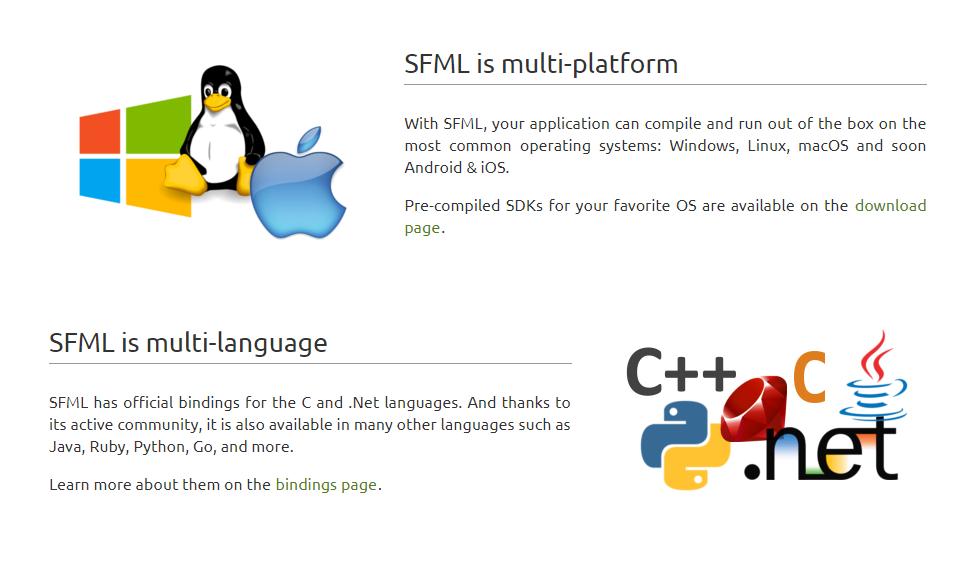
\includegraphics[scale=0.7]{images/sfmldetails}}
\caption{Chi tiết thư viện SFML. Nguồn: \url{gamedevspot.net}}
\end{figure}
\end{itemize}

\newpage

\section{Mô tả thiết kế phần mềm}
\subsection{Sơ đồ UML của phần mềm}
Do kích thước chiều ngang của giấy có hạn nên sơ đồ UML của phần mềm được đặt trong thư mục \textbf{UMLDiagram}, đính kèm với bản báo cáo này.

\subsection{Mô tả các lớp trong phần mềm}
\subsubsection{Namespace \lstinline{utilities}}
Namespace \lstinline{utilities} cung cấp các hàm bổ trợ cho quá trình xử lý, ví dụ như hàm cung cấp địa chỉ (location) của các hình ảnh, âm thanh, hay hàm kiểm tra vị trí hợp lệ...

\subsubsection{Lớp \lstinline{Settings}}
Lớp \lstinline{Settings} cung cấp một vài thông tin cài đặt cơ bản của game.\\
Sơ đồ UML của lớp \lstinline{Settings} như sau:

\begin{figure}[H]
\centering{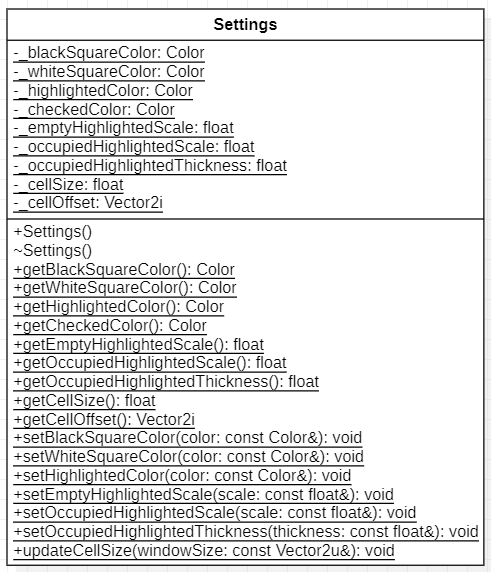
\includegraphics[scale=0.8]{images/classes/Settings}}
\caption{Sơ đồ UML của lớp \lstinline{Settings}}
\end{figure} 

Các thuộc tính (attributes) của lớp \lstinline{Settings} là thông tin về màu của các ô vuông trên bàn cờ, màu của ô vuông lúc được làm nổi bật (highlight), màu của ô vuông khi bị chiếu. Các màu này được dựa trên mã màu RGBA. Mã màu RGGA trong đồ án được lấy từ trang web: \url{https://rgbacolorpicker.com}. Ngoài ra, còn có các thuộc tính mô tả về tỉ lệ, độ dày mỏng của các nét highlight, cũng như kích thước và offset của ô vuông trên bàn cờ.\\
Các phương thức (methods) của lớp \lstinline{Settings} cung cấp các hàm getters và setters cho các thuộc tính của lớp.\\
Hầu hết các thuộc tính và phương thức của lớp \lstinline{Settings} (trừ hàm tạo $-$ constructor và hàm hủy $-$ destructor) đều được khai báo dưới dạng thuộc tính/phương thức tĩnh (\lstinline{method}), tạo ra sự tiện lợi khi ta cần gọi chúng, giúp ta không phải tạo một đối tượng mới mỗi khi muốn sử dụng đến các tính năng này.

\subsubsection{Các lớp enum}
\paragraph{Lớp enum \lstinline{GameSound}}
Lớp \lstinline{GameSound} cung cấp các loại âm thanh của game: âm thanh khi di chuyển quân cờ (MOVE), khi bắt quân (CAPTURE), khi chiếu (CHECK), khi chiếu hết (CHECKMATE) hay khi stalemate (trạng thái mà cả hai bên đều không còn nước nào có thể đi được).\\
Sơ đồ UML của lớp enum \lstinline{GameSound} như sau:
\begin{figure}[H]
\centering{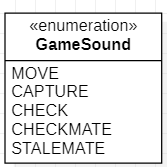
\includegraphics[scale=0.8]{images/classes/GameSound}}
\caption{Sơ đồ UML của lớp enum \lstinline{GameSound}}
\end{figure}

\paragraph{Lớp enum \lstinline{CellStatus}}
Lớp \lstinline{CellStatus} cung cấp các trạng thái của một ô vuông trên bàn cờ: đã có quân (OCCUPIED), chưa có quân (EMPTY) hay đang được highlight (HIGHLIGHTED).\\
Sơ đồ UML của lớp enum \lstinline{CellStatus} như sau:
\begin{figure}[H]
\centering{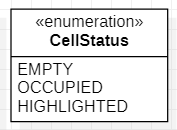
\includegraphics[scale=0.8]{images/classes/CellStatus}}
\caption{Sơ đồ UML của lớp enum \lstinline{CellStatus}}
\end{figure}

\paragraph{Lớp enum \lstinline{MoveType}}
Lớp \lstinline{MoveType} cung cấp thể loại của các nước di chuyển trong game: thăng cấp cho quân Tốt ($\mathrm{PROMOTION}$), nhập thành ngắn ($\mathrm{SHORT\_CASTLING}$), nhập thành dài ($\mathrm{LONG\_CASTLING}$), hoặc không phải các nước đi trên ($\mathrm{NONE}$).\\
Sơ đồ UML của lớp enum \lstinline{MoveType} như sau:
\begin{figure}[H]
\centering{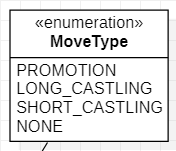
\includegraphics[scale=0.8]{images/classes/MoveType}}
\caption{Sơ đồ UML của lớp enum \lstinline{MoveType}}
\end{figure}

\paragraph{Lớp enum \lstinline{PieceType}}
Lớp \lstinline{PieceType} cung cấp các loại quân cờ: quân Vua (KING), quân Hậu (QUEEN), quân Tượng (BISHOP), quân Mã (KNIGHT), quân Xe (ROOK) và quân Tốt (PAWN).\\
Sơ đồ UML của lớp enum \lstinline{PieceType} như sau:
\begin{figure}[H]
\centering{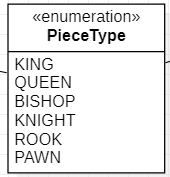
\includegraphics[scale=0.8]{images/classes/PieceType}}
\caption{Sơ đồ UML của lớp enum \lstinline{PieceType}}
\end{figure}

\paragraph{Lớp enum \lstinline{PieceDirection}}
Lớp \lstinline{PieceDirection} cung cấp hướng di chuyển thẳng về phía trước cho quân Tốt: đi lên (UP) đối với Tốt trắng và đi xuống (DOWN) đối với Tốt đen.\\
Sơ đồ UML của lớp enum \lstinline{PieceDirection} như sau:
\begin{figure}[H]
\centering{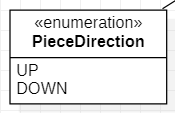
\includegraphics[scale=0.8]{images/classes/PieceDirection}}
\caption{Sơ đồ UML của lớp enum \lstinline{PieceDirection}}
\end{figure}

\paragraph{Lớp enum \lstinline{PieceColor}}
Lớp \lstinline{PieceColor} cho biết hai màu của người chơi/quân cờ: màu trắng (WHITE) và màu đen (BLACK).\\
Sơ đồ UML của lớp enum \lstinline{PieceColor} như sau:
\begin{figure}[H]
\centering{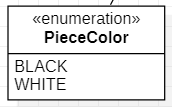
\includegraphics[scale=0.8]{images/classes/PieceColor}}
\caption{Sơ đồ UML của lớp enum \lstinline{PieceColor}}
\end{figure}

\subsubsection{Lớp \lstinline{ChessMove}}
Lớp \lstinline{ChessMove} cung cấp thông tin về nước đi trên bàn cờ.\\
Sơ đồ UML của lớp \lstinline{ChessMove} như sau:
\begin{figure}[H]
\centering{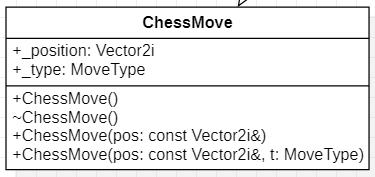
\includegraphics[scale=0.8]{images/classes/ChessMove}}
\caption{Sơ đồ UML của lớp \lstinline{ChessMove}}
\end{figure}
Các thuộc tính của lớp \lstinline{ChessMove} cho biết vị trí và thể loại của nước đi đó.\\
Các phương thức khởi tạo của lớp \lstinline{ChessMove} cho phép ta khởi tạo mặc định, khởi tạo với một tham số và khởi tạo với đầy đủ tham số.

\subsubsection{Lớp \lstinline{Cell}}
Lớp \lstinline{Cell} thể hiện mỗi một ô vuông trên bàn cờ vua.\\
Sơ đồ UML của lớp \lstinline{Cell} như sau:
\begin{figure}[H]
\centering{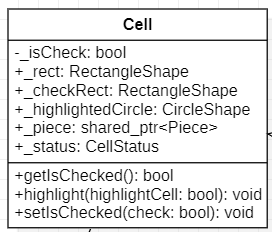
\includegraphics[scale=0.8]{images/classes/Cell}}
\caption{Sơ đồ UML của lớp \lstinline{Cell}}
\end{figure}
Các thuộc tính chính của lớp \lstinline{Cell} gồm có thuộc tính để đánh dấu xem ô này có đang bị chiếu hay không, một con trỏ \lstinline{shared_ptr} trỏ đến một đối tượng thuộc lớp \lstinline{Piece} (sẽ được trình bày trong phần sau) $-$ quân cờ hiện tại ở ô này (nếu ô này đang không bị chiếm giữ bởi quân cờ nào  thì trỏ đến \lstinline{nullptr}), hay thuộc tính thể hiện trạng thái hiện tại của ô vuông này. Ngoài ra, các đối tượng từ lớp \lstinline{RectangleShape} và \lstinline{CircleShape} của thư viện SFML cũng được sử dụng để tạo các thuộc tính nhằm phục vụ cho việc thiết kế giao diện người dùng (GUI).\\
Thuộc tính \lstinline{_piece} có kiểu con trỏ \lstinline{shared_ptr} của thư viện STL để hạn chế tình trạng rò rỉ bộ nhớ (memory leak).

\subsubsection{Lớp \lstinline{Piece}}
Lớp \lstinline{Piece} là một lớp trừu tượng, để biểu diễn một quân cờ tổng quát trên bàn cờ vua.\\
Sơ đồ UML của lớp \lstinline{Piece} như sau:
\begin{figure}[H]
\centering{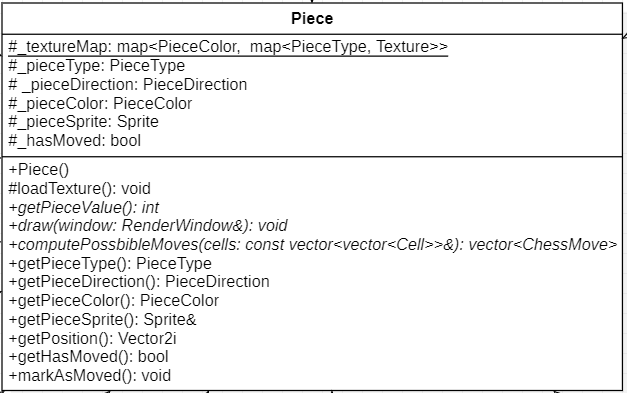
\includegraphics[scale=0.8]{images/classes/Piece}}
\caption{Sơ đồ UML của lớp \lstinline{Piece}}
\end{figure}
Các thuộc tính của lớp \lstinline{Piece} được khai báo \lstinline{protected} để cho các lớp kế thừa từ nó có thể truy cập vào các thuộc tính.\\
Lớp \lstinline{Piece} có thuộc tính tĩnh \lstinline{_textureMap} lưu trữ các \lstinline{Texture} của lần lượt từng quân cờ của mỗi màu. Lớp \lstinline{Texture} và \lstinline{Sprite} được sử dụng từ thư viện SFML.\\
Các thuộc tính khác thể hiện màu sắc, loại quân cờ, hướng di chuyển cùng với một thuộc tính để kiểm tra xem quân cờ này đã di chuyển hay chưa.\\
Lớp này cung cấp các getters, setters cho các thuộc tính, phương thức dùng để tải (load) các Texture. Ngoài ra, lớp \lstinline{Piece} còn cung cấp các phương thức thuần ảo nhằm tận dụng tính đa hình (polymorphism). Các phương thức thuần ảo này sẽ được cài đặt trong các lớp kế thừa cho phù hợp.\\
Trong các lớp kế thừa từ lớp \lstinline{Piece} (6 lớp được trình bày tiếp theo), các thuật toán tìm nước đi khả dĩ (possible moves) của quân cờ được lấy từ: \url{https://github.com/mbusy/chess/tree/master/src}.

\subsubsection{Lớp \lstinline{King}}
Lớp \lstinline{King} là một lớp con kế thừa từ lớp \lstinline{Piece}, thể hiện quân Vua trên bàn cờ. Do là một lớp kế thừa nên nó kế thừa lại tất cả các thuộc tính và phương thức của lớp \lstinline{Piece}. Các phương thức thuần ảo của lớp \lstinline{Piece} được viết lại trong lớp \lstinline{King}.\\
Sơ đồ UML của lớp \lstinline{King} như sau:
\begin{figure}[H]
\centering{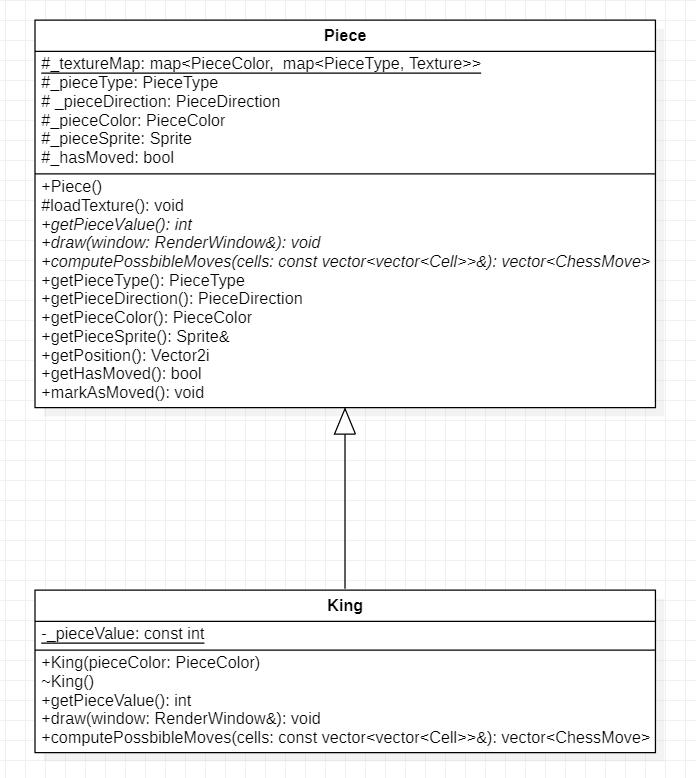
\includegraphics[scale=0.6]{images/classes/King}}
\caption{Sơ đồ UML của lớp \lstinline{King}}
\end{figure}
Hình sau mô tả các nước đi có thể của quân Vua, được viết trong phương thức \lstinline{computePossibleMoves}.
\begin{figure}[H]
\centering{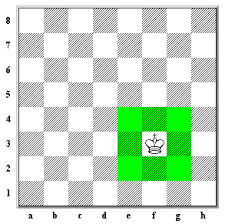
\includegraphics[scale=0.6]{images/moves/King}}
\caption{Các nước đi của quân Vua. Nguồn: \url{chesscorner.com}}
\end{figure}

\subsubsection{Lớp \lstinline{Queen}}
Lớp \lstinline{Queen} là một lớp con kế thừa từ lớp \lstinline{Piece}, thể hiện quân Hậu trên bàn cờ. Do là một lớp kế thừa nên nó kế thừa lại tất cả các thuộc tính và phương thức của lớp \lstinline{Piece}. Các phương thức thuần ảo của lớp \lstinline{Piece} được viết lại trong lớp \lstinline{Queen}.\\
Sơ đồ UML của lớp \lstinline{Queen} như sau:
\begin{figure}[H]
\centering{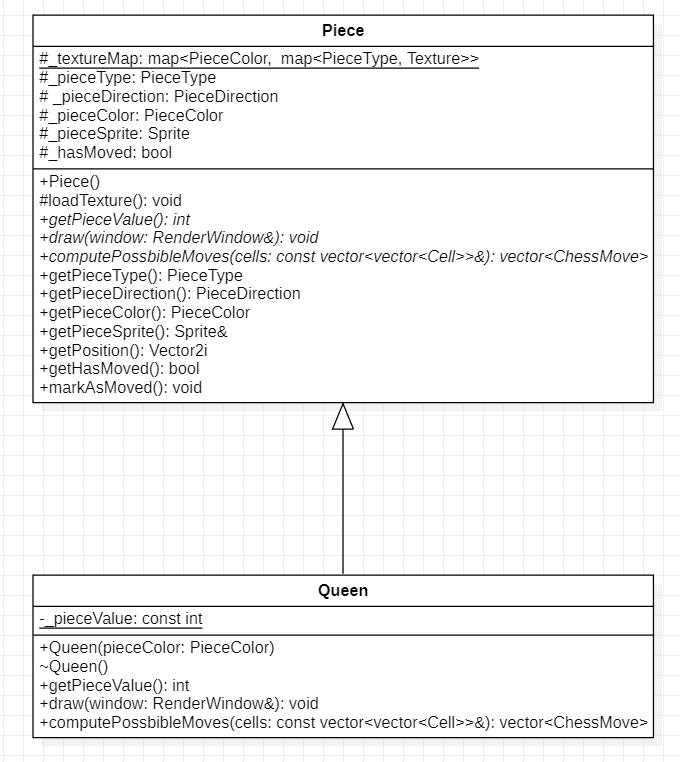
\includegraphics[scale=0.6]{images/classes/Queen}}
\caption{Sơ đồ UML của lớp \lstinline{Queen}}
\end{figure}
Hình sau mô tả các nước đi có thể của quân Hậu, được viết trong phương thức \lstinline{computePossibleMoves}.
\begin{figure}[H]
\centering{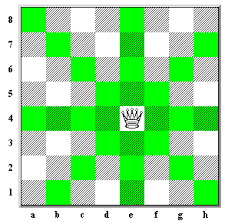
\includegraphics[scale=0.6]{images/moves/Queen}}
\caption{Các nước đi của quân Hậu. Nguồn: \url{chesscorner.com}}
\end{figure}

\subsubsection{Lớp \lstinline{Bishop}}
Lớp \lstinline{Bishop} là một lớp con kế thừa từ lớp \lstinline{Piece}, thể hiện quân Tượng trên bàn cờ. Do là một lớp kế thừa nên nó kế thừa lại tất cả các thuộc tính và phương thức của lớp \lstinline{Piece}. Các phương thức thuần ảo của lớp \lstinline{Piece} được viết lại trong lớp \lstinline{Bishop}.\\
Sơ đồ UML của lớp \lstinline{Bishop} như sau:
\begin{figure}[H]
\centering{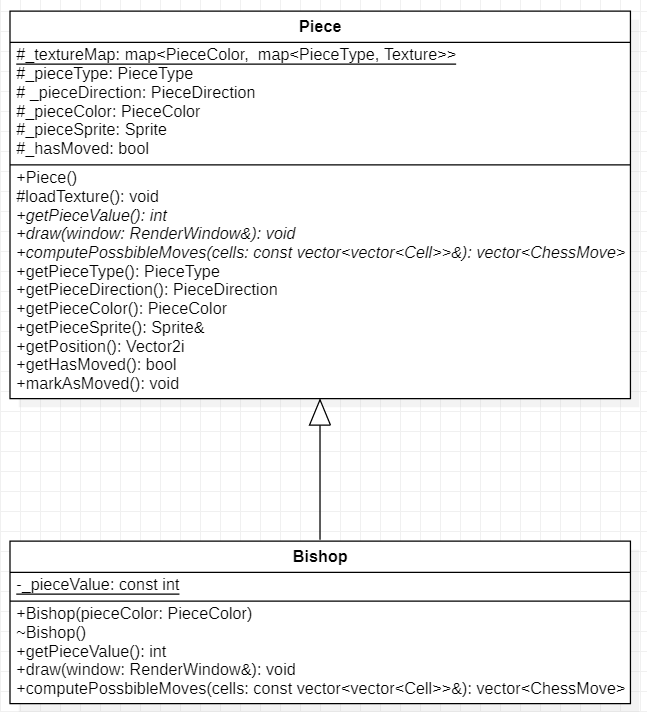
\includegraphics[scale=0.6]{images/classes/Bishop}}
\caption{Sơ đồ UML của lớp \lstinline{Bishop}}
\end{figure}
Hình sau mô tả các nước đi có thể của quân Tượng, được viết trong phương thức \lstinline{computePossibleMoves}.
\begin{figure}[H]
\centering{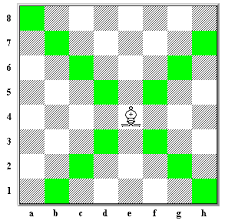
\includegraphics[scale=0.6]{images/moves/Bishop}}
\caption{Các nước đi của quân Tượng. Nguồn: \url{chesscorner.com}}
\end{figure}

\subsubsection{Lớp \lstinline{Knight}}
Lớp \lstinline{Knight} là một lớp con kế thừa từ lớp \lstinline{Piece}, thể hiện quân Mã trên bàn cờ. Do là một lớp kế thừa nên nó kế thừa lại tất cả các thuộc tính và phương thức của lớp \lstinline{Piece}. Các phương thức thuần ảo của lớp \lstinline{Piece} được viết lại trong lớp \lstinline{Knight}.\\
Sơ đồ UML của lớp \lstinline{Knight} như sau:
\begin{figure}[H]
\centering{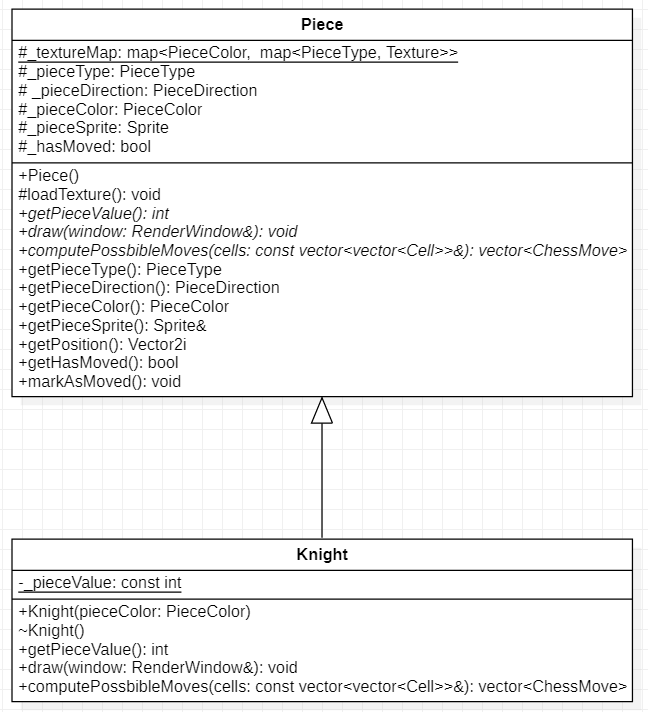
\includegraphics[scale=0.6]{images/classes/Knight}}
\caption{Sơ đồ UML của lớp \lstinline{Knight}}
\end{figure}
Hình sau (các ô màu đỏ) mô tả các nước đi có thể của quân Mã, được viết trong phương thức \lstinline{computePossibleMoves}.
\begin{figure}[H]
\centering{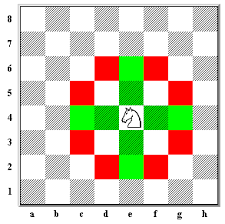
\includegraphics[scale=0.6]{images/moves/Knight}}
\caption{Các nước đi của quân Mã. Nguồn: \url{chesscorner.com}}
\end{figure}

\subsubsection{Lớp \lstinline{Rook}}
Lớp \lstinline{Rook} là một lớp con kế thừa từ lớp \lstinline{Piece}, thể hiện quân Xe trên bàn cờ. Do là một lớp kế thừa nên nó kế thừa lại tất cả các thuộc tính và phương thức của lớp \lstinline{Piece}. Các phương thức thuần ảo của lớp \lstinline{Piece} được viết lại trong lớp \lstinline{Rook}.\\
Sơ đồ UML của lớp \lstinline{Rook} như sau:
\begin{figure}[H]
\centering{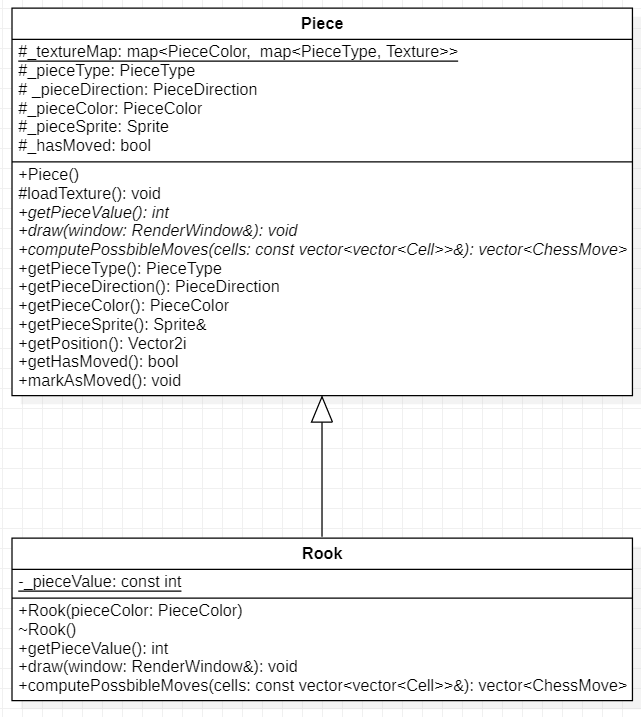
\includegraphics[scale=0.6]{images/classes/Rook}}
\caption{Sơ đồ UML của lớp \lstinline{Rook}}
\end{figure}
Hình sau mô tả các nước đi có thể của quân Xe, được viết trong phương thức \lstinline{computePossibleMoves}.
\begin{figure}[H]
\centering{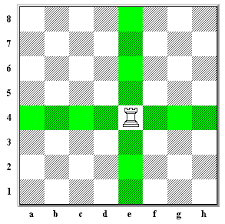
\includegraphics[scale=0.6]{images/moves/Rook}}
\caption{Các nước đi của quân Xe. Nguồn: \url{chesscorner.com}}
\end{figure}

\subsubsection{Lớp \lstinline{Pawn}}
Lớp \lstinline{Pawn} là một lớp con kế thừa từ lớp \lstinline{Piece}, thể hiện quân Tốt trên bàn cờ. Do là một lớp kế thừa nên nó kế thừa lại tất cả các thuộc tính và phương thức của lớp \lstinline{Piece}. Các phương thức thuần ảo của lớp \lstinline{Piece} được viết lại trong lớp \lstinline{Pawn}.\\
Sơ đồ UML của lớp \lstinline{Pawn} như sau:
\begin{figure}[H]
\centering{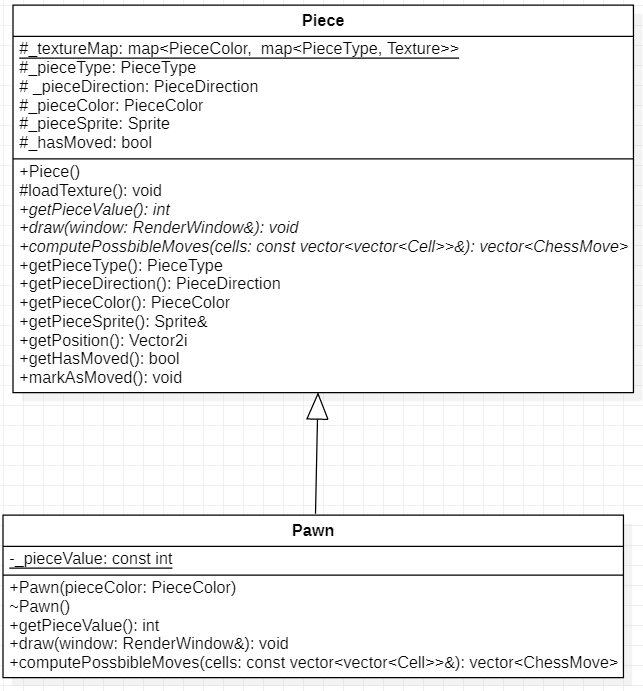
\includegraphics[scale=0.6]{images/classes/Pawn}}
\caption{Sơ đồ UML của lớp \lstinline{Pawn}}
\end{figure}
Hình sau mô tả các nước đi có thể của quân Tốt, được viết trong phương thức \lstinline{computePossibleMoves}.
\begin{figure}[H]
\centering{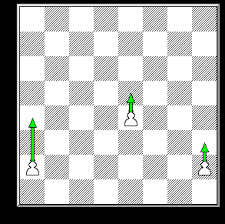
\includegraphics[scale=0.6]{images/moves/Pawn}}
\caption{Các nước đi của quân Tốt. Nguồn: \url{chesscorner.com}}
\end{figure}
Việc phong cấp cho quân Tốt sẽ được xử lý ở lớp \lstinline{ChessBoard}, được trình bày ở phần sau.

\subsubsection{Lớp \lstinline{AudioPlayer}}
Lớp \lstinline{AudioPlayer} chủ yếu cung cấp cho ta các phương thức liên quan đến việc xử lý âm thanh của game (load, play, pause, resume, stop).\\
Sơ đồ UML của lớp \lstinline{AudioPlayer} như sau:
\begin{figure}[H]
\centering{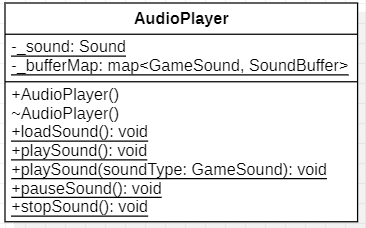
\includegraphics[scale=0.6]{images/classes/AudioPlayer}}
\caption{Sơ đồ UML của lớp \lstinline{AudioPlayer}}
\end{figure}

\subsubsection{Lớp \lstinline{GameUser}}
Lớp \lstinline{GameUser} thể hiện người dùng game Cờ vua (bên trắng và bên đen).\\
Sơ đồ UML của lớp \lstinline{GameUser} như sau:
\begin{figure}[H]
\centering{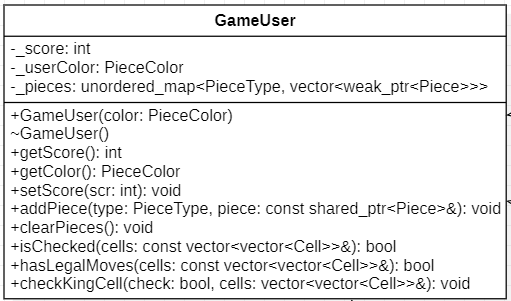
\includegraphics[scale=0.6]{images/classes/GameUser}}
\caption{Sơ đồ UML của lớp \lstinline{GameUser}}
\end{figure}
Các thuộc tính của lớp \lstinline{GameUser} gồm có điểm, màu, và các quân cờ. Con trỏ \lstinline{weak_ptr} của thư viện STL được sử dụng để tham chiếu đến đối tượng được quản lý bởi \lstinline{shared_ptr}.\\
Các thuộc tính của lớp \lstinline{GameUser} bao gồm các getters, setters, các hàm giúp ta thêm các quân cờ, kiểm tra xem người dùng có đang bị chiếu hay không, kiểm tra xem người dùng còn nước đi hợp lệ nào hay không, hay phương thức dùng để chiếu người dùng.

\subsubsection{Lớp \lstinline{ChessBoard}}
Lớp \lstinline{ChessBoard} thể hiện bàn cờ của game Cờ vua trên cửa sổ game.\\
Sơ đồ UML của lớp \lstinline{ChessBoard} như sau:
\begin{figure}[H]
\centering{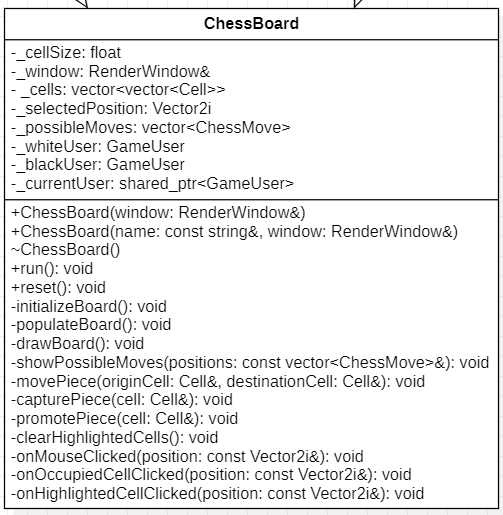
\includegraphics[scale=0.6]{images/classes/ChessBoard}}
\caption{Sơ đồ UML của lớp \lstinline{ChessBoard}}
\end{figure}
Các thuộc tính chủ yếu của lớp \lstinline{ChessBoard} gồm cửa sổ game, mảng hai chiều các ô vuông trên bàn cờ, các nước đi có thể có, người chơi màu trắng, người chơi màu đen và người chơi hiện tại của game.\\
Các phương thức có tầm vực \lstinline{public} của lớp \lstinline{ChessBoard} gồm các phương thức \lstinline{run()}, là phương thức chủ yếu để biểu diễn bàn cờ lên GUI, và phương thức \lstinline{reset()} dùng để reset bàn cờ.\\
Ngoài ra, lớp \lstinline{ChessBoard} còn gồm nhiều phương thức có tầm vực \lstinline{private}:
\begin{itemize}
 \item Phương thức \lstinline{initializeBoard}, dùng để khởi tạo một bàn cờ.
 \item Phương thức \lstinline{populateBoard}, dùng để đặt các quân cờ vào vị trí trên bàn cờ.
  \item Phương thức \lstinline{drawBoard}, dùng để hiển thị bàn cờ ra màn hình.
  \item Phương thức \lstinline{showPossibleMoves}, dùng để hiển thị những nước đi khả dĩ của quân cờ được chọn hiện tại.
  \item Phương thức \lstinline{movePiece}, dùng để di chuyển một quân cờ.
  \item Phương thức \lstinline{capturePiece}, dùng để bắt (ăn) một quân cờ khác.
  \item Phương thức \lstinline{promotePiece}, dùng để phong cấp cho quân Tốt khi đạt đủ điều kiện.
  \item Ngoài ra, còn các phương thức xử lý những cú click chuột trên cửa sổ game.
\end{itemize} 
Phần cài đặt của lớp \lstinline{ChessBoard} sử dụng nhiều các lớp và phương thức của chúng trong thư viện SFML.
\newpage

\section{Mô tả tính năng của phần mềm}
Đồ án Game Cờ vua 2 người cung cấp một phần mềm mô phỏng môn thể thao trí tuệ Cờ vua, với tính năng 2 người chơi. Phần mềm cung cấp đầy đủ các tính năng cơ bản của một game cờ vua như các bước di chuyển, tính năng bắt quân, chiếu, phong cấp cho quân Tốt, nhập thành...\\
Phần mềm được thiết kế và xây dựng trên nền tảng Linux (Ubuntu 20.04), vì vậy, những tính năng sau đây cũng được ví dụ trên nền tảng này.

\subsection{Màn hình khởi động của game}
Hình sau đây là màn hình khởi động của game, với đầy đủ các quân cờ đã được sắp xếp vào vị trí, sẵn sàng cho một trận chiến mới.
\begin{figure}[H]
\centering{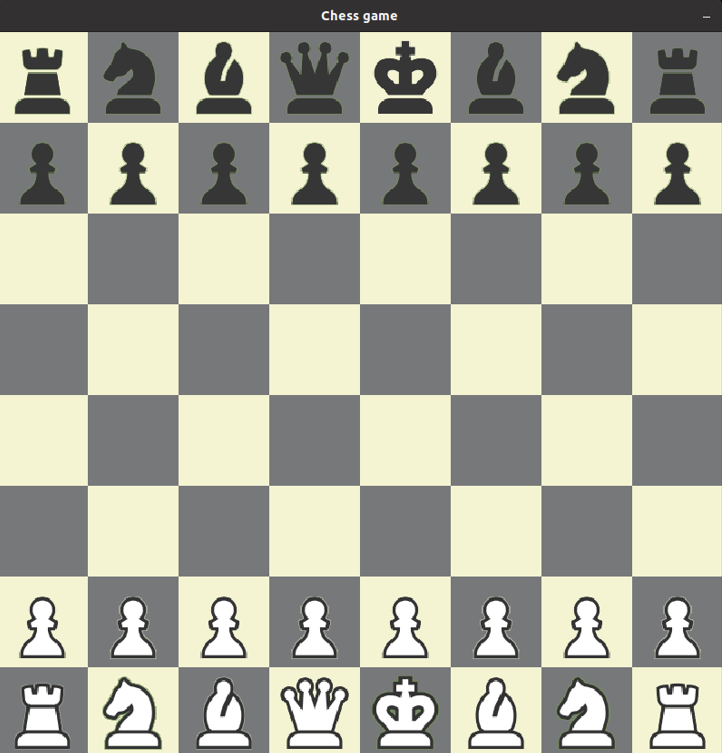
\includegraphics[scale=0.5]{images/features/Start}}
\caption{Màn hình khởi động của game}
\end{figure}

\subsection{Di chuyển quân cờ}
Hình sau đây là nước đi đầu tiên trong game, với quân Tốt trắng tiến lên hai bước.
\begin{figure}[H]
\centering{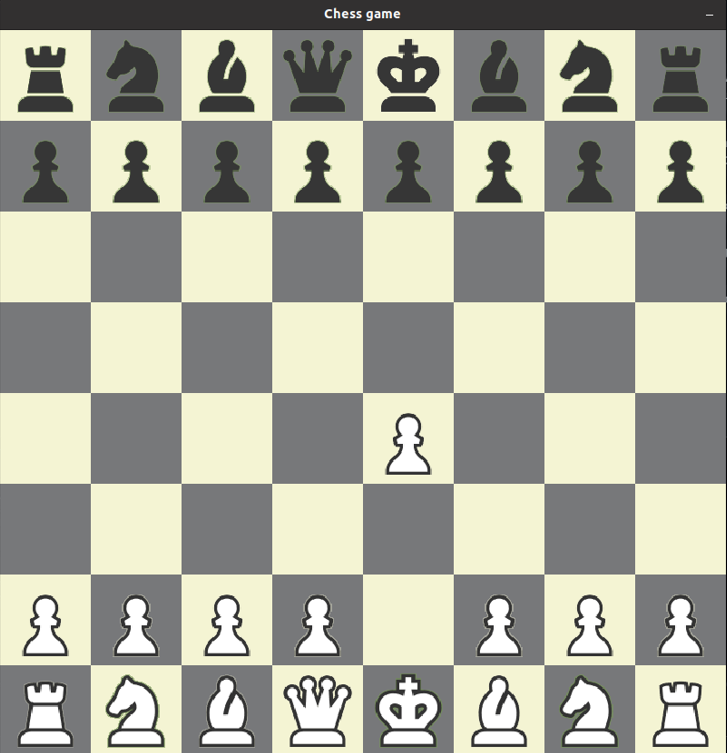
\includegraphics[scale=0.5]{images/features/FirstMove}}
\caption{Di chuyển quân cờ trong game}
\end{figure}

\subsection{Tính năng bắt (ăn) quân}
Hình sau đây là ví dụ về tính năng bắt quân theo đường chéo của quân Tốt trắng đối với quân Tốt đen, sau khi quân Tốt đen này tiến vào ô có thể bị bắt bởi quân Tốt trắng. Quân cờ bị bắt sẽ bị loại khỏi bàn chơi ngay lập tức.
\begin{figure}[H]
\centering{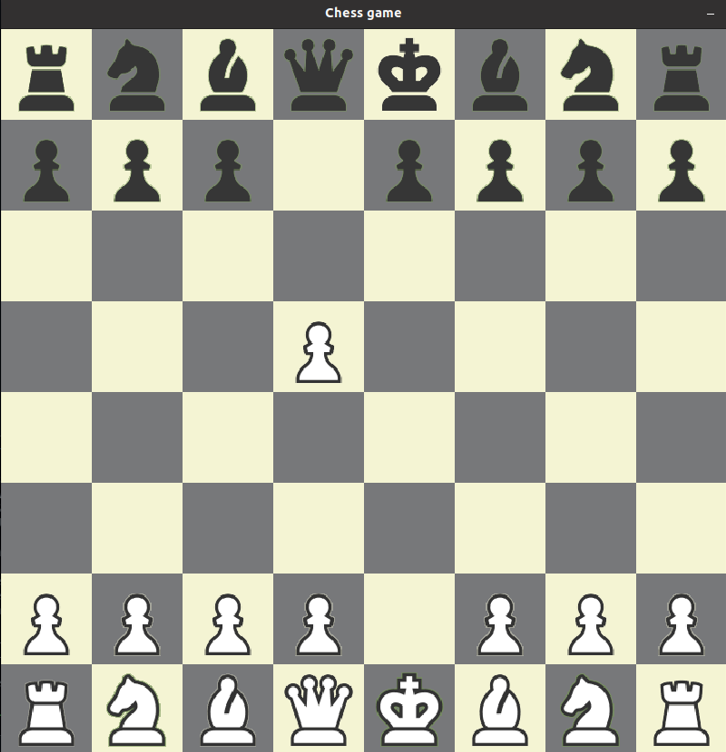
\includegraphics[scale=0.5]{images/features/Capture}}
\caption{Bắt quân cờ của đối thủ}
\end{figure}

\subsection{Chiếu}
Hình sau đây mô tả tình huống quân Vua bị chiếu, tức là quân Vua nằm trong một ô có thể bị bắt ở các quân cờ của đối thủ. Ô bị chiếu hiện tại sẽ được tô màu đỏ. Sau khi bị chiếu, quân Vua phải di chuyển đến nơi an toàn, hoặc những quân cờ khác phải di chuyển để "cắt" đường chiếu của quân cờ đối thủ, thậm chí có thể bắt quân cờ này để bảo vệ vua. Nếu không thể, ván đấu sẽ kết thúc và bên bị chiếu sẽ thua cuộc.
\begin{figure}[H]
\centering{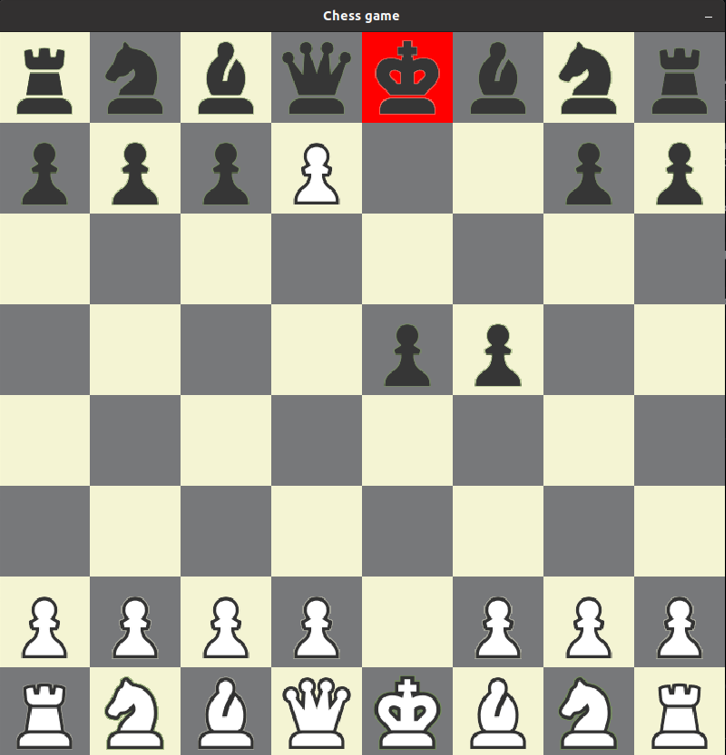
\includegraphics[scale=0.5]{images/features/Check}}
\caption{Chiếu}
\end{figure}

\subsection{Thăng cấp (Phong cấp) cho quân Tốt}
Khi quân Tốt tiến đến hàng cuối cùng trên "địa phận" của đối thủ, nó sẽ được thăng cấp thành một trong bốn quân: Hậu, Xe, Tượng, Mã. Hình sau đây mô tả một ví dụ về tính năng thăng cấp cho quân Tốt này.
\begin{figure}[H]
\centering{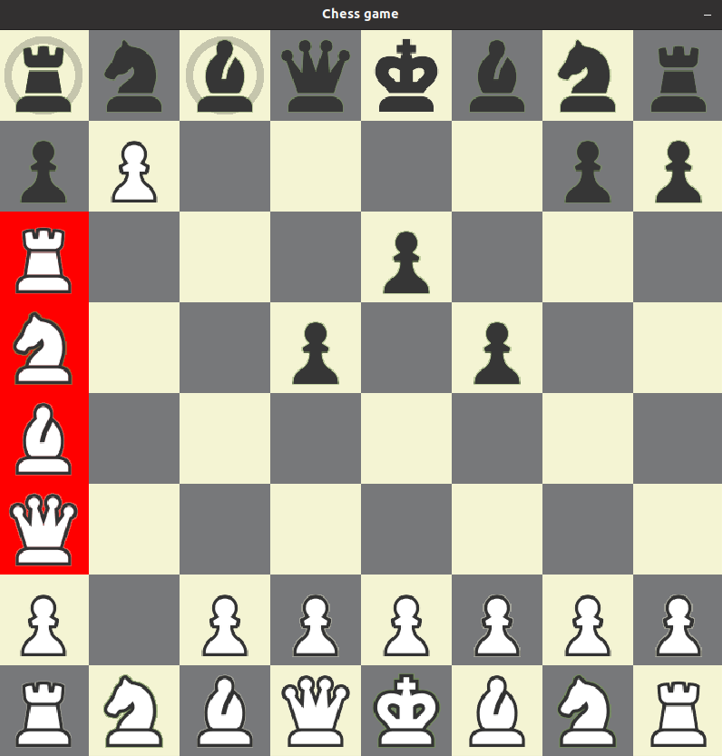
\includegraphics[scale=0.5]{images/features/Promote}}
\caption{Thăng cấp cho quân Tốt}
\end{figure}

\subsection{Nhập thành}
Khi quân Vua và quân Xe của một bên chưa di chuyển, các ô giữa chúng đều trở thành ô trống và ô đích đến không bị chiếu thì quân Vua có thể tiến hành nhập thành. Có hai loại nhập thành, ứng với hai quân Xe, lần lượt là long castling (tạm dịch là "nhập thành dài") $-$ ứng với quân Xe ở xa Vua hơn và short castling (tạm dịch là "nhập thành ngắn) $-$ ứng với quân Xe ở gần Vua hơn. Hình sau đây cho ta một ví dụ về nhập thành dài.
\begin{figure}[H]
\centering{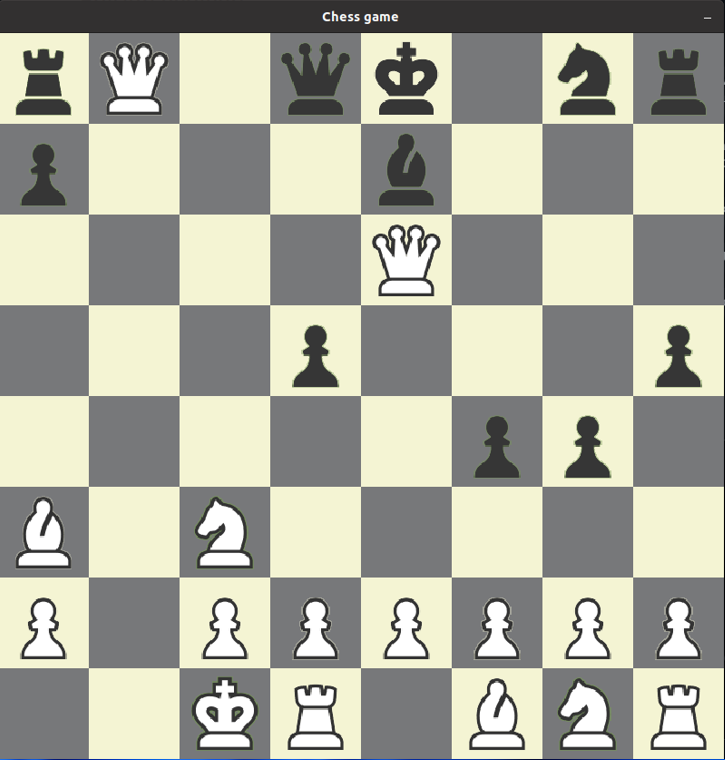
\includegraphics[scale=0.5]{images/features/Castling}}
\caption{Nhập thành}
\end{figure}

\subsection{Kết thúc ván đấu (chiếu hết)}
Khi quân Vua bị chiếu và không còn nước đi nào khác có thể "cứu" quân Vua ra khỏi ô bị chiếu này, ván đấu sẽ kết thúc với chiến thắng cho bên chiếu. Hình sau đây cho ta một ví dụ về bàn cờ lúc kết thúc ván đấu.
\begin{figure}[H]
\centering{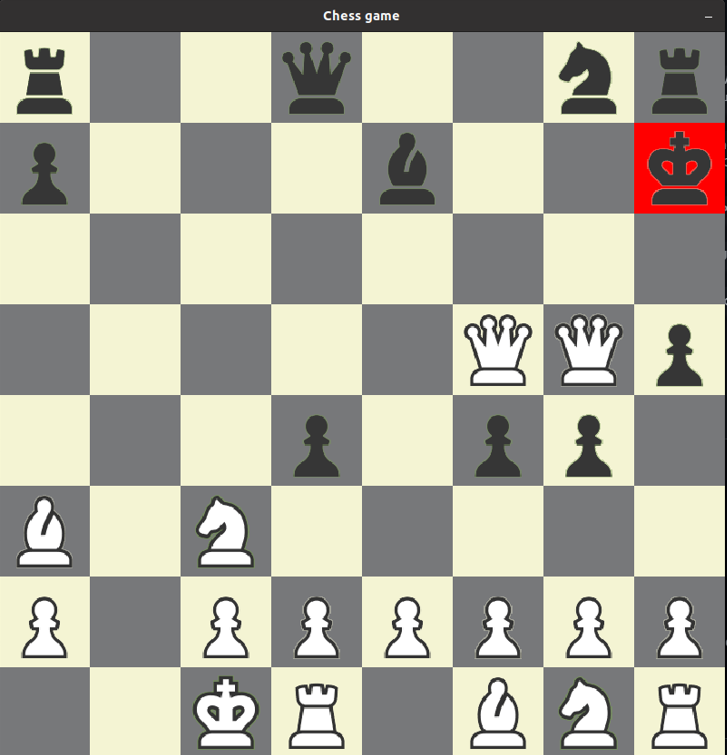
\includegraphics[scale=0.5]{images/features/Checkmate}}
\caption{Kết thúc ván đấu (chiếu hết)}
\end{figure}
Khi tình huống này xảy ra, một thông báo sẽ hiện lên màn hình console, cho ta biết người chiến thắng.
\begin{figure}[H]
\centering{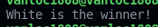
\includegraphics[scale=3]{images/features/Winner}}
\caption{Thông báo người chiến thắng}
\end{figure}

\subsection{Thoát game}
Ta có thể thoát game bằng cách tắt cửa sổ game hoặc nhấn phím Escape (Esc) ở góc trên bên trái bàn phím.
\newpage

\section{Hướng dẫn build phần mềm}
Phần mềm được thiết kế và xây dựng cho môi trường Linux, cho nên phần hướng dẫn này chỉ tập trung hướng dẫn build phần mềm trên môi trường này.\\
Trước tiên, để build phần mềm trên môi trường này, chúng ta cần cài đặt thư viện SFML cho Linux bằng câu lệnh:
\begin{lstlisting}
sudo apt-get install libsfml-dev
\end{lstlisting} 
Nếu câu lệnh trên không hoạt động, ta có thể cài đặt thư viện này bằng những cách khác theo hướng dẫn trong link sau: \url{https://www.sfml-dev.org/tutorials/2.5/start-linux.php}\\
Do phần mềm đã hỗ trợ Makefile, nên sau khi cài đặt thư mục SFML thành công, ta chỉ cần mở thư mục chứa source code và dùng lệnh:
\begin{lstlisting}
make
\end{lstlisting}
Sau khi hoàn thành, tập tin thực thi có tên là \textbf{chess} sẽ xuất hiện. Ta chỉ cần dùng lệnh sau để khởi chạy tập tin này:
\begin{lstlisting}
./chess
\end{lstlisting}
\newpage

\section{Demo của phần mềm}
Nhóm đã tiến hành quay video demo của phần mềm, gồm có sơ đồ UMl, giới thiệu các file trong source code, hướng dẫn build phần mềm, demo một ván đấu cờ vua.\\
Link demo phần mềm: \url{https://youtu.be/Pev0-ZqRduw}
\newpage

\section{Nhận xét về đồ án}
\subsection{Ưu điểm}
\subsubsection{Mô tả tính năng phần mềm}
Báo cáo đã mô tả đầy đủ các tính năng của phần mềm.

\subsubsection{Mô tả thiết kế phần mềm}
Sơ đồ UML của phần mềm và mô tả các lớp đã được trình bày trong báo cáo và hình ảnh sơ đồ UML đính kèm.

\subsubsection{Các kỹ thuật của lập trình hướng đối tượng}
Đồ án đã ứng dụng được nhiều kỹ thuật trong lập trình hướng đối tượng.
\begin{itemize}
\item Hàm dựng (constructor): hầu hết các lớp đều được xây dựng với ít nhất một hàm dựng.
\item Hàm hủy (destructor): các lớp sử dụng các lớp con trỏ "an toàn" của thư viện STL nên hầu hết các hàm hủy đều được để ở dạng mặc định, nhưng chúng cũng được khai báo một cách tường minh trong lớp.
\item Tính đóng gói (encapsulation): các lớp đều tuân thủ tính đóng gói của lập trình hướng đối tượng, tuân theo quy tắc hộp đen và quy tắc "Tell, don't ask".
\item Tính kế thừa (inheritance): ứng dụng được mối quan hệ tổng quát hóa/đặc biệt hóa (IS-A, generalization), mối quan hệ bao hàm/bộ phận (association), đặc biệt là mối quan hệ bao hàm/bộ phận độc lập (aggregation).
\item Tính đa hình (polymorphism): ứng dụng được tính đa hình trong việc xây dựng các phương thức của các quân cờ.
\item Phương thức thuần ảo (pure virtual method): ứng dụng được hàm thuần ảo trong lớp \lstinline{Piece}. 
\item Lớp trừu tượng (abstract class): tạo dựng lớp \lstinline{Piece} là lớp trừu tượng, các lớp kế thừa từ \lstinline{Piece} sẽ khai báo các phương thức thuần ảo của lớp \lstinline{Piece}.
\item Sử dụng kỹ thuật try-throw-catch, giúp phát hiện và xử lý lỗi và ngoại lệ (exception).
\end{itemize}

\subsubsection{Các cấu trúc dữ liệu}
Các cấu trúc dữ liệu sử dụng trong đồ án hầu hết đều từ thư viện STL, giúp ta xử lý nhanh chóng và tránh tình trạng rò rỉ bộ nhớ (memory leak).

\subsubsection{Giao diện}
Đồ án đã xây dựng một giao diên người dùng (GUI) trực quan, sinh động, minh họa đầy đủ các tính năng của môn Cờ vua.

\subsubsection{Độ hoàn thành}
Đồ án đã hoàn thành hầu hết các chỉ tiêu đặt ra.

\subsubsection{Trình bày}
Báo cáo đã trình bày rõ ràng, chi tiết về đồ án.

\subsubsection{Design pattern}
Đồ án đã ứng dụng mẫu thiết kế Iterator trong quá trình duyệt qua các phần tử của nhiều cấu trúc dữ liệu khác nhau.

\subsection{Khuyết điểm}
Trong quá trình xây dựng, nhóm đã thử tính năng đánh với máy (sử dụng stockfish) nhưng đã gặp lỗi và chưa cung cấp được.\\
Chưa thiết kế được cơ sở dữ liệu hỗ trợ quản lý tài khoản, nên tính năng quản lý tài khoản chưa được đưa vào phần mềm.\\
Chưa cung cấp tính năng đi lại cho các nước đi trong ván cờ.
\newpage

\section{Hướng phát triển}
Nghiên cứu áp dụng lại stockfish hoặc một engine khác để xây dựng tính năng chơi với máy, giúp việc luyện tập cờ vua trở nên dễ dàng hơn với người sử dụng.\\
Nghiên cứu xây dựng cơ sở dữ liệu cho việc quản lý tài khoản.\\
Nghiên cứu xây dựng tính năng cho phép người chơi đi lại sau mỗi nước đi.\\
Nghiên cứu cải tiến giao diện người dùng, cung cấp nhiều tính năng hơn nữa.
\newpage

\section{Phân công công việc của các thành viên}
Bảng \ref{jobs} dưới đây mô tả thông tin phân công các thành viên của nhóm.
\begin{longtable}{|c| p{0.5\textwidth}|c|} 
\hline 
Thành viên & Công việc & Phần trăm đóng góp \\ 
\hline 
Nguyễn Văn Lộc & \begin{itemize}
\item Lên ý tưởng thiết kế cho phần mềm.
\item Xây dựng các lớp Pawn, Cell, AudioPlayer, GameSound, ChessMove, ChessBoard, Settings.
\item Thiết kế giao diện người dùng (GUI) cho phần mềm.
\item Tester chính cho phần mềm.
\item Viết báo cáo chính cho phần mềm.
\end{itemize} & 34 \\ 
\hline 
Nguyễn Nhật Tiến & \begin{itemize}
\item Tham gia thiết kế sơ đồ UML của chương trình.
\item Tham gia viết báo cáo cho phần mềm.
\item Xây dựng các lớp Knight, Rook, ChessBoard.
\item Tìm kiếm tài nguyên hình ảnh, âm thanh cho phần mềm.
\end{itemize} & 21 \\ 
\hline 
Trà Như Khuyên & \begin{itemize}
\item Tham gia thiết kế sơ đồ UML của chương trình.
\item Tham gia viết báo cáo cho phần mềm.
\item Xây dựng các lớp Piece, King, GameUser, ChessBoard. \item Tham gia xây dựng namespace Utility.
\end{itemize} & 23 \\ 
\hline 
Nguyễn Minh Tâm & \begin{itemize}
\item Tham gia thiết kế sơ đồ UML của chương trình.
\item Tham gia viết báo cáo cho phần mềm.
\item Xây dựng các lớp Queen, Bishop, ChessBoard.
\item Tham gia xây dựng namespace Utility.
\end{itemize} & 22 \\ 
\hline 
\caption{Bảng phân công thành viên}
\label{jobs}
\end{longtable} 

\newpage

\section{Phiếu tự đánh giá}
Bảng \ref{points} dưới đây là phiếu tự đánh giá các tiêu chí của nhóm.
\begin{longtable}{|c| p{0.6\textwidth}|c|c|} 
\hline 
STT & Tiêu chí & Điểm & Đánh giá \\ 
\hline 
1 & Tài liệu mô tả phần mềm & 0.5 & 0.5 \\ 
\hline 
2 & Tài liệu thiết kế phần mềm & 3 & 3 \\ 
\hline 
3 & Ứng dụng được ít nhất 5 kỹ thuật đã học trong môn Phương pháp lập trình hướng đối tượng & 3 & 3 \\ 
\hline 
4 & Giao diện đẹp & 1 & 0.75 \\ 
\hline 
5 & Độ hoàn thiện & 1 & 0.75 \\ 
\hline 
6 & Trình bày & 1 & 0.75 \\ 
\hline 
7 & Cơ sở dữ liệu & 0.5 & 0 \\ 
\hline 
8 & Ứng dụng được ít nhất một mẫu design pattern & 1 & 0.5 \\ 
\hline 
& Tổng điểm & 11 & 10 \\ 
\hline 
\caption{Bảng tự đánh giá}
\label{points}
\end{longtable} 
\newpage

\section*{Lời cảm ơn}
Những kiến thức về lập trình hướng đối tượng được ứng dụng trong đồ án của chúng em được Thầy Nguyễn Minh Huy giảng dạy rất nhiệt tình, tâm huyết. Trong quá trình thực hiện đồ án, chúng em đã nhận được những sự hướng dẫn, những góp ý tận tâm của Thầy Trần Anh Duy. Chúng em xin cảm ơn hai Thầy vì đồ án này nói riêng và vì những kiến thức mà hai Thầy đã cung cấp nói chung ạ.\\
Bên cạnh đó, trong quá trình thực hiện đồ án, nhóm đã nhận được những lời góp ý từ các bạn cùng lớp. Nhóm xin gửi lời cảm ơn chân thành đến các bạn.\\
Ngoài ra, nhóm cũng đã tham khảo từ nhiều trang web như GitHub, trang web chính thức của thư viện SFML. Những thuật toán, những ý kiến giải đáp trên các diễn đàn trên đã góp phần giúp nhóm thực hiện đồ án này. 
\begin{flushright}
Thành phố Hồ Chí Minh, tháng 1 năm 2022
\end{flushright}

\end{document}